\chapter{Installation and Usage}
\section{Software Requirements}
For development following software components are needed:

\begin{itemize}
	\item Java (JDK) 1.6 or 1.7
	\item Maven
  \item Eclipse (Juno)
	\item Maven Plugin for Eclipse
  \item Git or Egit for Eclipse
  \item Modelbus Team Provider for Eclipse
	\item Modelbus 1.9.7
	\item Metrino for Modelbus with following plugins
		\begin{itemize}
			\item Metrino rule evaluator plugin
			\item Metrino measure plugin
		\end{itemize}
\end{itemize}
Sonar will be downloaded and deployed via Maven at compile time.

\section{Installation Manual}
In the following sections we explain every detail. Just skip a section if you think you still have done that what the regarding section focuses. 



\subsection{Java}
We tested the software with Java 1.6 and 1.7. You can get those from \href{http://www.oracle.com/technetwork/java/javase/downloads/index.html}{here}. Select and download the current JDK to install it on your system. If Java is ready, make sure that the following system variables exist:
\begin{verbatim}
JAVA_HOME = C:\Program Files\Java\jdk1.7.0_09
(change the path to your JDK install path)
\end{verbatim}

Also you must add your JAVA\_HOME variable (add \textbackslash bin\textbackslash ) to your path variable.
\begin{verbatim}
PATH =...;%JAVA_HOME%\bin\;
\end{verbatim}



\subsection{Maven}
Download the current Maven from \href{http://maven.apache.org/download.html}{here} and follow the instructions from the README: Extract it somewhere and create following path variables:
\begin{verbatim}
M2_HOME = C:\Program Files\apache-maven-3.0.4 
(change the path to your maven folder)
M2 = %M2_HOME%\bin\
PATH =...;%M2%;
\end{verbatim}



\subsection{Eclipse}
Download Eclipse from \href{http://www.eclipse.org/juno/}{here}.
We recommend a current Eclipse version. We use Eclipse Juno (4.2) for Java developer.
Remember to select the correct version for your operating system. 



\subsection{Maven Plugin for Eclipse}
Open Eclipse and open "Help | Install New Software...". Now select or add the repository of your eclipse version. In our example we will use 

\url{http://download.eclipse.org/releases/juno}
 
Select "m2e – Maven Integration for Eclipse" and click through the progress to install the plugin. If everything works well, Eclipse will ask you for an Eclipse restart. 

\begin{figure}
	\centering
		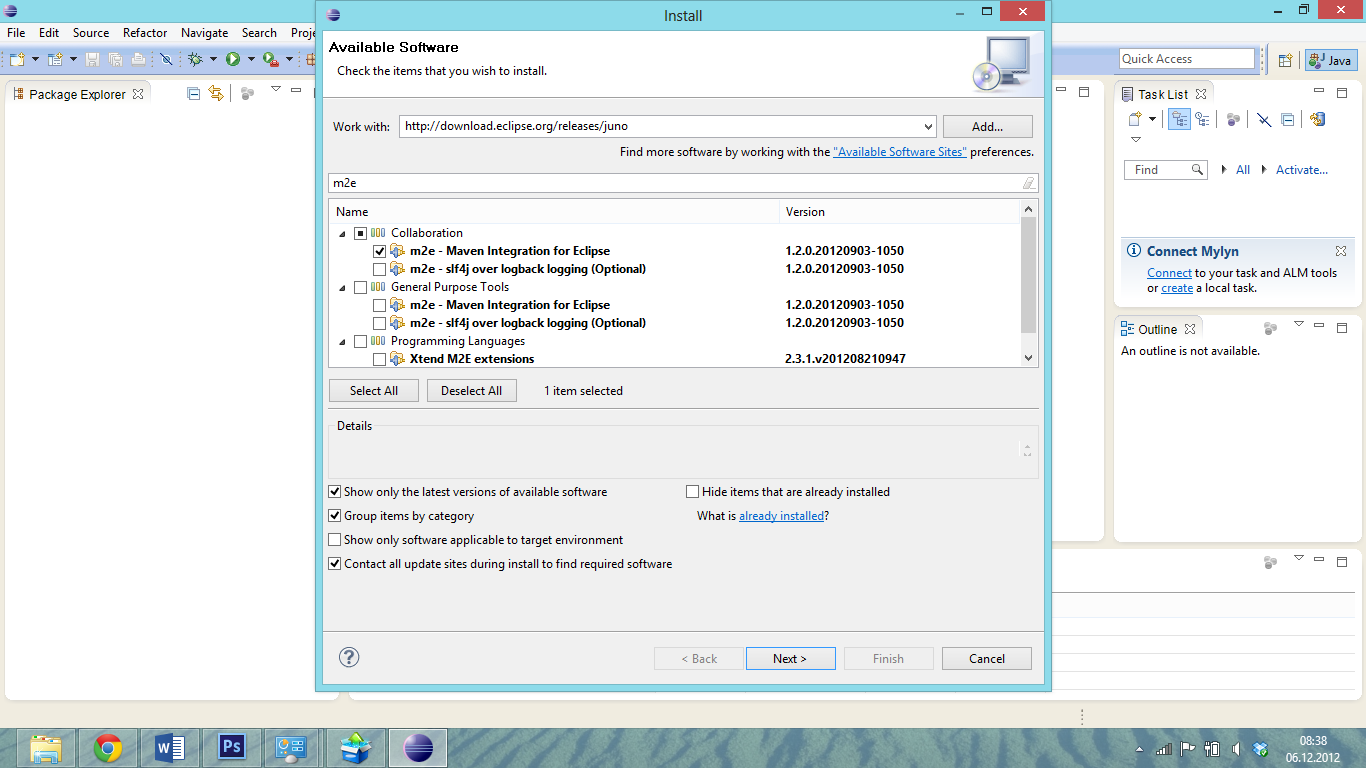
\includegraphics[width=\textwidth]{m2eplugin}
	\caption{Maven Eclipse plugin installation}
	\label{fig:m2eplugin}
\end{figure}




\subsection{Git or Egit for Eclipse}
If you have installed Juno, Egit is already integrated. If not so, you can download Egit from \href{http://download.eclipse.org/egit/updates}{here}. Or you get and install Git from \href{http://git-scm.com/download/}{here}.
	


\subsection{Modelbus Team Provider for Eclipse}
The update site for the Modelbus Team Provider is \href{http://www.modelbus.org/modelbus/downloads/current/site}{here}. Select only the ModelBus Team Provider for the installation.



\subsection{Modelbus and Metrino}
Request \href{http://www.modelbus.org/modelbus/}{the Modelbus developers} for a version of Modelbus with an integrated Metrino service. Make sure that the following Jars lie in the plugin folder of Modelbus:
\begin{itemize}
	\item de.fraunhofer.fokus.metrino.ruleEvaluator
	\item de.fraunhofer.fokus.metrino.measure
\end{itemize}
Extract Modelbus to any location in your file system. Now you have to setup the configuartaion file of Modelbus. Open the "modelbus.config" in the "serverConfiguration" folder of your modelbus installation. Set the "repositoryLocation" to "http://localhost:8080/modelbusrepository" and the "svnRepositoryLocation" to "repository":
\begingroup
    \fontsize{10pt}{12pt}\selectfont
    \begin{verbatim}  
<?xml version="1.0" encoding="UTF-8"?>
<config:ConfigModel xmi:version="2.0" xmlns:xmi="http://www.omg.org/XMI" 
  xmlns:config="http://www.modelbus.org/system/model/config.ecore">
  <locations name="repositoryLocation" location="http://localhost:8080/modelbusrepository"/>
<!-- <locations name="secureRepositoryLocation" location="https://0.0.0.0:8181/modelbusrepository">
    <properties name="SSLTrustStore" value="SSL/cacerts.jks"/>
    <properties name="SSLTrustStorePassword" value="password"/>
    <properties name="SSLKeyStore" value="SSL/modelbus.keystore"/>
    <properties name="SSLKeyStorePassword" value="password"/>
    <properties name="SSLAlgorithm" value="RSA"/>
    <properties name="SSLPassword" value="password"/>
  </locations> //-->
  <locations name="notificationLocation" location="tcp://localhost:61616"/>
  <locations name="svnRepositoryLocation" location="repository"/>
</config:ConfigModel>
    \end{verbatim}  
\endgroup
Then you will have to set some environment variables. Set
\begin{itemize}
	\item MODELBUS\_ROOT to the folder of your Modelbus installation
	\item MODELBUS\_NOTIFICATION\_LOCATION  to "tcp://localhost:61616" like in the config file
	\item MODELBUS\_REPOSITORY\_LOCATION to \\
	"http://localhost:8080/modelbusrepository" like in the config file
\end{itemize}



\section{Usage Manual}

The typical workflow for plugin development is:
\begin{enumerate}
	\item start Modelbus
	\item open the plugin project with Eclipse 
	\item make some changes to the code
	\item build the project with the Maven goal "install"
	\item deploy Sonar including out plugin via Maven
	\item analyse the project with the goal "sonar:sonar" to test the plugin on your installed Modelbus repository
\end{enumerate}

The typical workflow for an user of our plugin is:
\begin{enumerate}
	\item start ModelBus
	\item start Sonar with our plugin via Maven
	\item check in models into the Modelbus repository
	\item analyse a Maven project with the goal "sonar:sonar" (this will also analyse your installed Modelbus repository)
\end{enumerate}

The single steps are described below in detail.



\subsection{Download the source of our Sonar-Modelbus-Plugin}
Download the following copy of our repository:

\url{https://github.com/arsenij-solovjev/sonar-modelbus-plugin/archive/master.zip}

Extract the archive and if you like copy the folder sonar-modelbus-plugin-master into a special folder. It is just important that you don't copy this folder in your Eclipse workspace.



\subsection{Start Modelbus}
Under Windows start the "startModelBusServer.exe" of your Modelbus installation.

Under Linux run the "startup.sh" as root user. Make sure that the "startup.sh" and the "bin/service" files are executable.

If Modelbus is up, you can visit the Modelbus manager under \url{http://localhost:8080/modelbus?startup=manager}: You can login with the username "Admin" and the password "ModelBus". Here you can see all the checked in files and models. When uploading a new file, press the refresh button to see the changes.

\begin{figure}
	\centering
		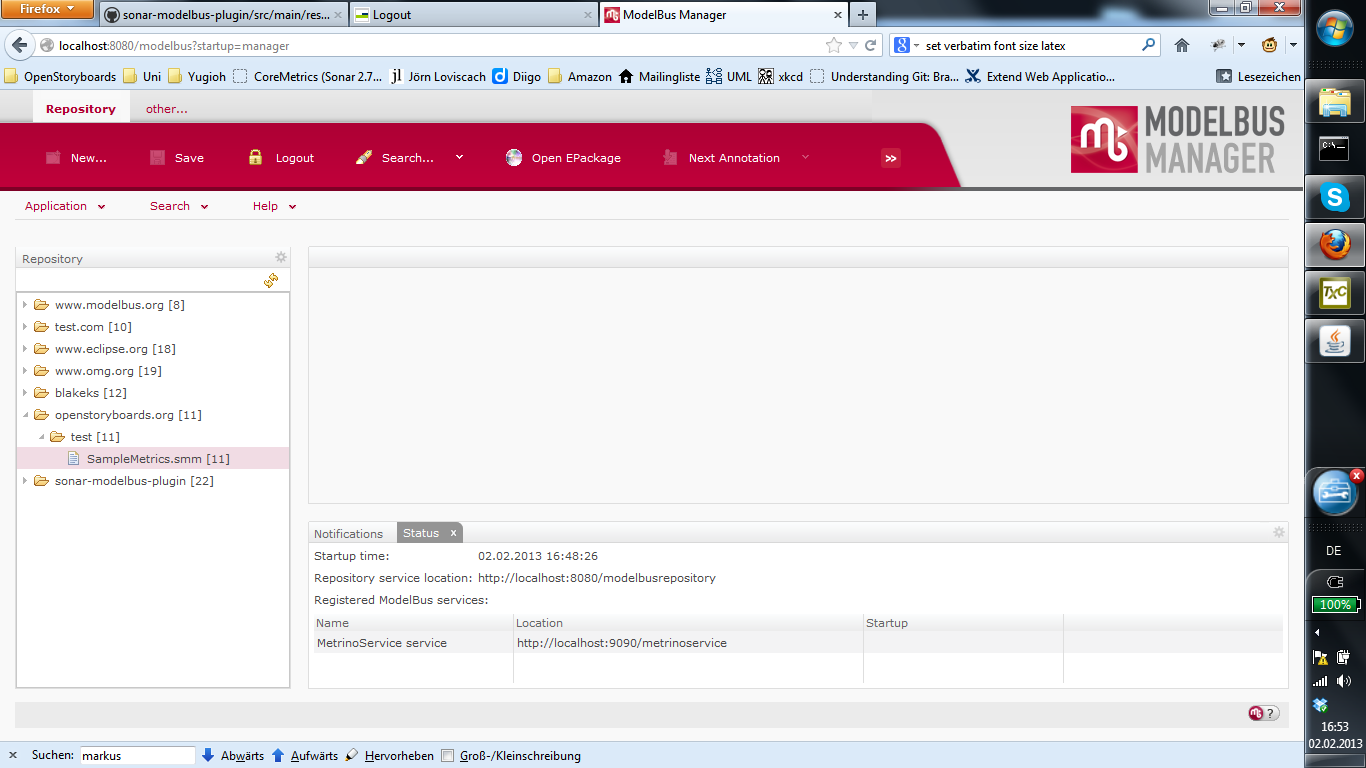
\includegraphics[width=\textwidth]{modelbusmanager}
	\caption{The Modelbus manager}
	\label{fig:modelbusmanager}
\end{figure}


\subsection{Uploading models}
We created a tool for checking in and out files from/to the ModelBus repository. It can be simply called via "make". First compile the tool: Go to the "modelbusclient/sonar-modelbus-client" folder and run:
\begin{verbatim}
make install
\end{verbatim}
This will compile and package the tool. Next, checkin some models to the Modelbus repository using:
\begin{verbatim}
make checkin 
  URI=http://uri.de/location/in/repository/file.txt 
  FILENAME=location/to/local/file.txt
\end{verbatim}
You can find some example models in the "/src/main/resources/metrinostuff" folder of our plugin.


\subsection{Create a new Eclipse project}
Now create a new Eclipse project:

\begin{figure}
	\centering
		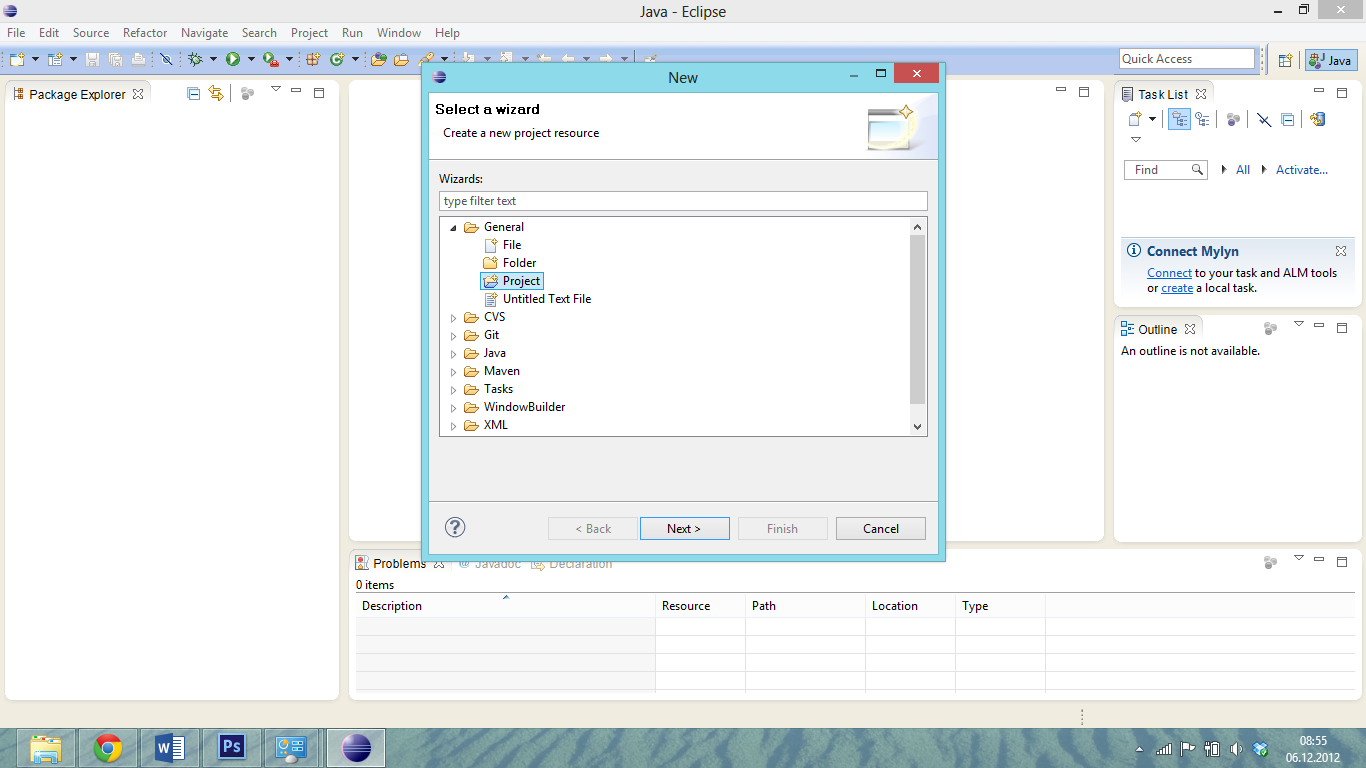
\includegraphics[width=\textwidth]{neweclipseproject}
	\caption{Creating a new Eclispe project}
	\label{fig:neweclipseproject}
\end{figure}

Unselect the "Use default location" box and select the sonar-modelbus-plugin-master folder. Don't forget to set a project name.
 
\begin{figure}
	\centering
		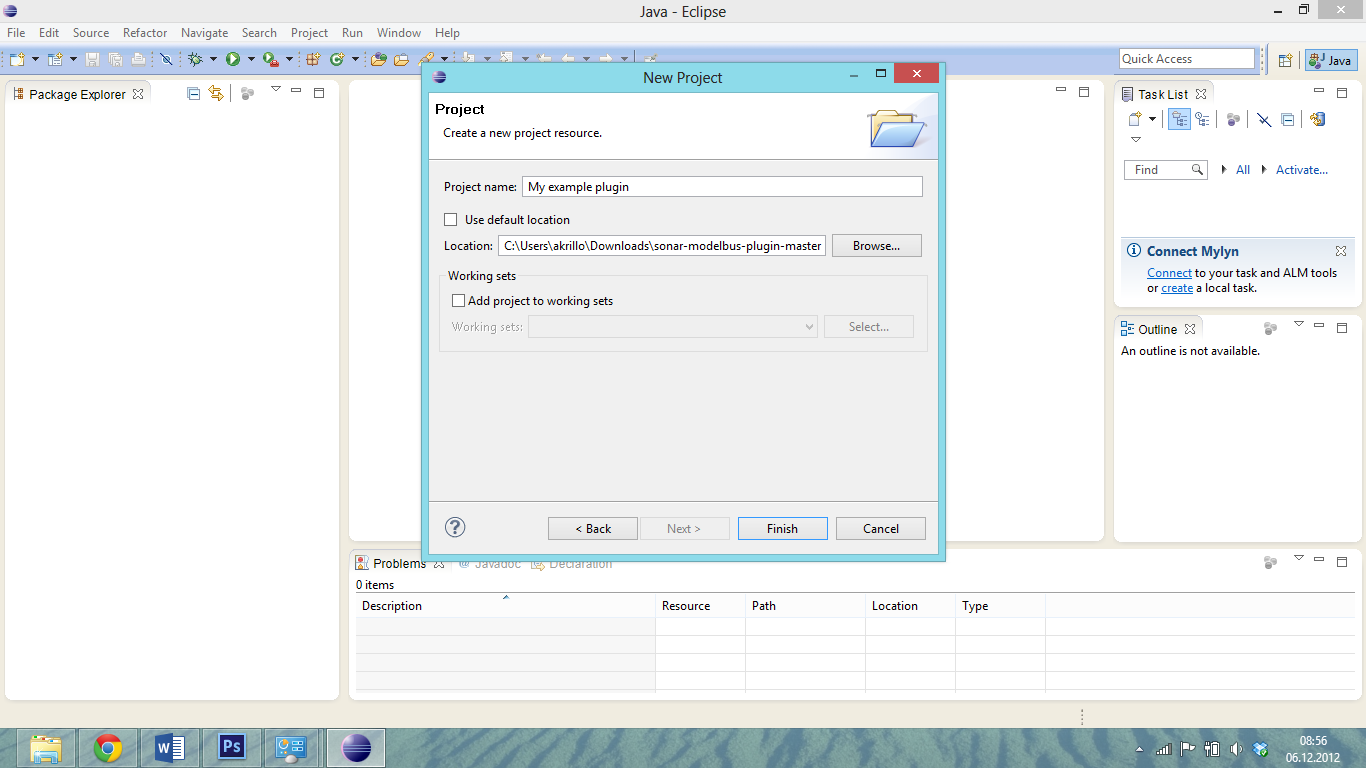
\includegraphics[width=\textwidth]{selectlocation}
	\caption{Selecting a location}
	\label{fig:selectlocation}
\end{figure}

Notice: If you finish the project creation process you may get
"Git could not detect where GIT is installed" or "check HOME directory" warning but it doesn't matter in this case.



\subsection{Convert your project to a Maven project}
Right click on your project folder and choose "Configure | Convert to Maven Project".
 
\begin{figure}
	\centering
		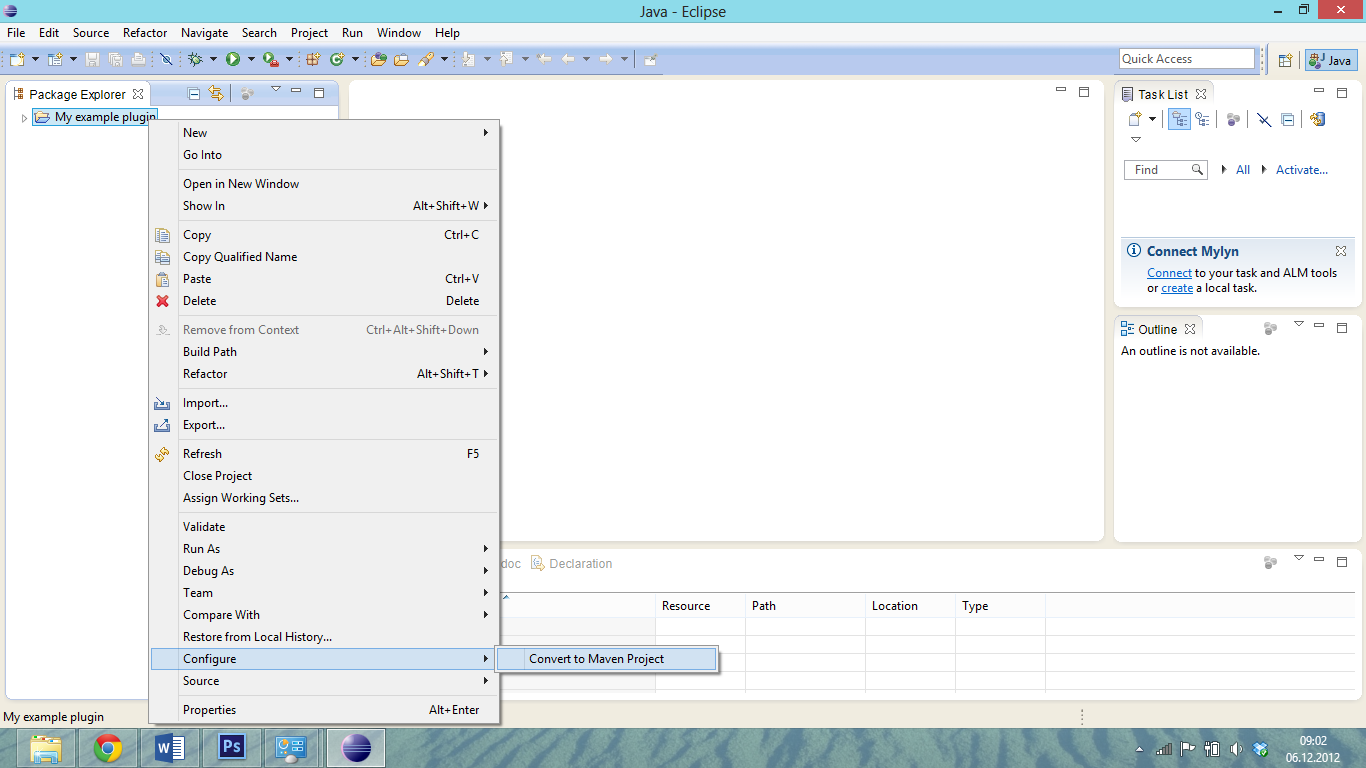
\includegraphics[width=\textwidth]{converttomavenproject}
	\caption{Converting to a Maven project}
	\label{fig:converttomavenproject}
\end{figure}

Notice: If you get any errors (this is not unusual) just ignore them. If you can't do the next step just repeat the previous one.



\subsection{Compilation}
Next: right click on your project again and select "Run as | Maven install".
\begin{figure}
	\centering
		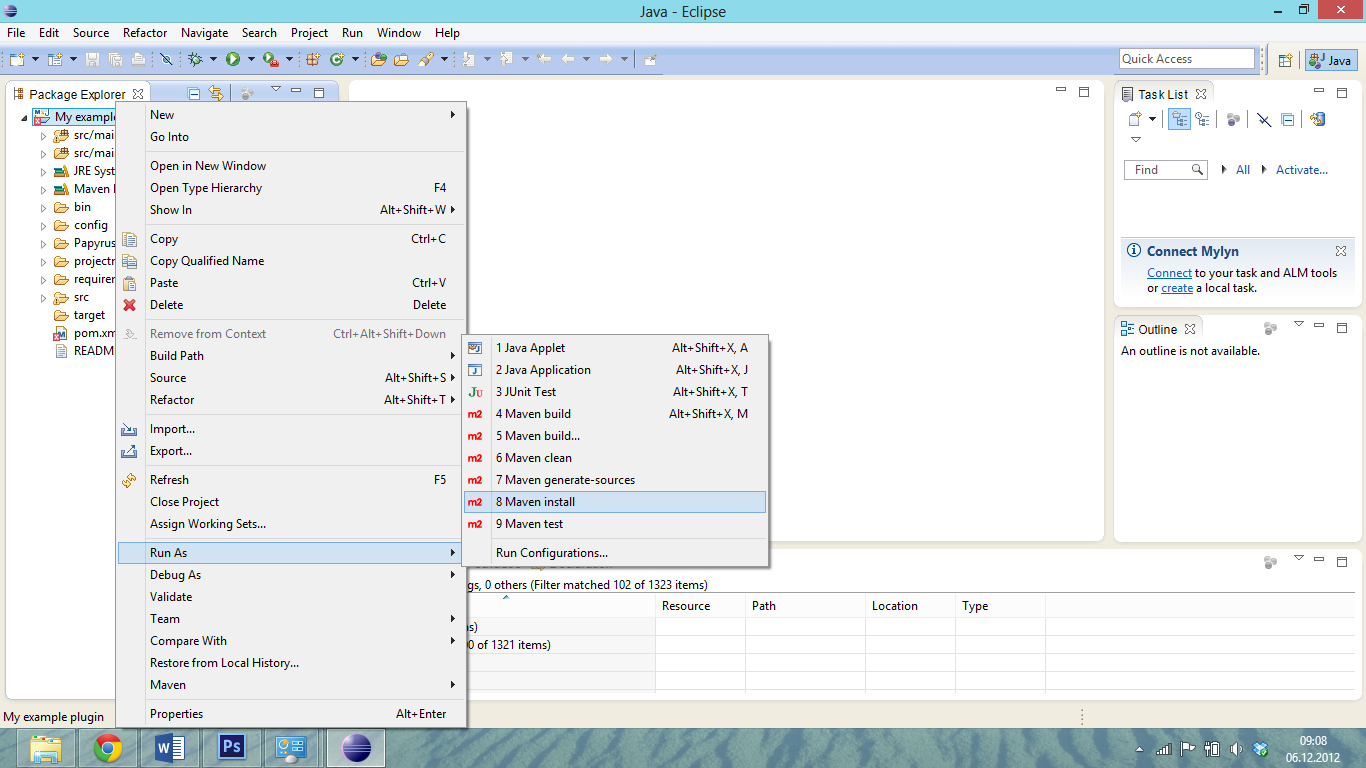
\includegraphics[width=\textwidth]{maveninstall}
	\caption{Maven install}
	\label{fig:maveninstall}
\end{figure} 
If everything works well you see a "BUILD SUCCESS" reports like this:
\begin{figure}
	\centering
		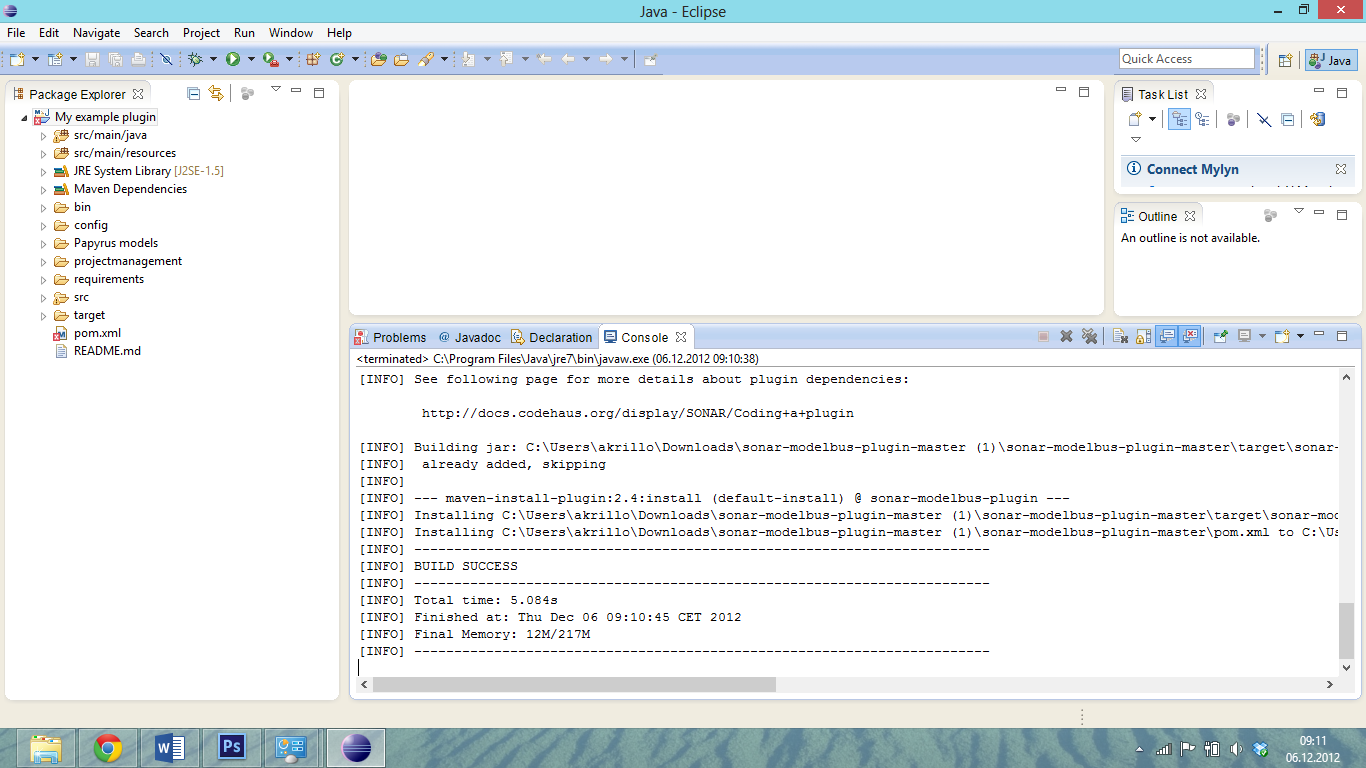
\includegraphics[width=\textwidth]{buildsuccess}
	\caption{BUILD SUCCESS}
	\label{fig:buildsuccess}
\end{figure}



\subsection{Deploy the Sonar server}
To run Sonar with our example plugin we need to run maven with an other goal. Right click on your Project and select "Run as | Maven Build". In "Goals" you must copy-paste 
\begin{verbatim}
org.codehaus.sonar:sonar-dev-maven-plugin::start-war
-Dsonar.runtimeVersion=3.3
\end{verbatim}
Then press "Run" to start the build process that will deploy a Sonar server for you. 

\begin{figure}
	\centering
		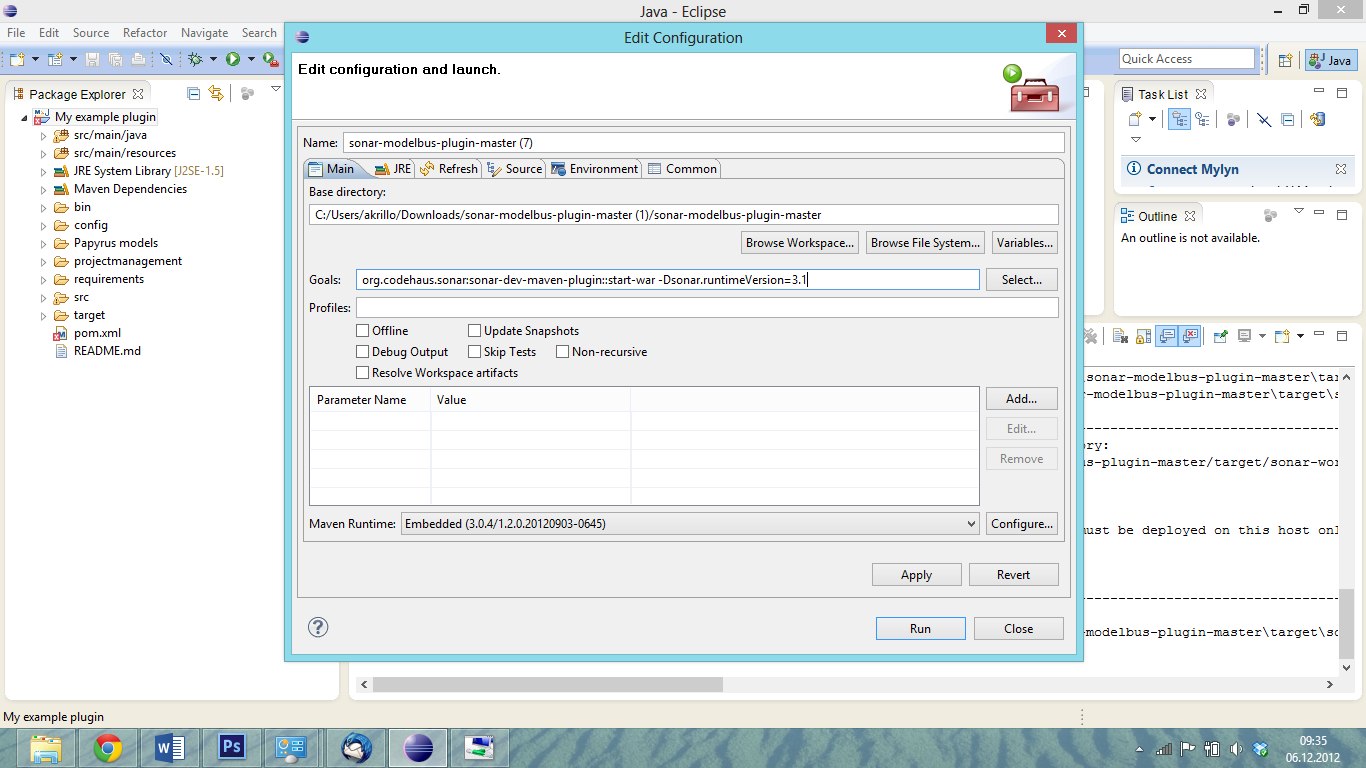
\includegraphics[width=\textwidth]{sonardeploy}
	\caption{Deploying Sonar with Maven}
	\label{fig:sonardeploy}
\end{figure}
 
Notice: this can take some minutes and if it seems to be frozen just restart the build process. If some errors occur just restart.
If everything went fine you will see following status messages:
 
\begin{figure}
	\centering
		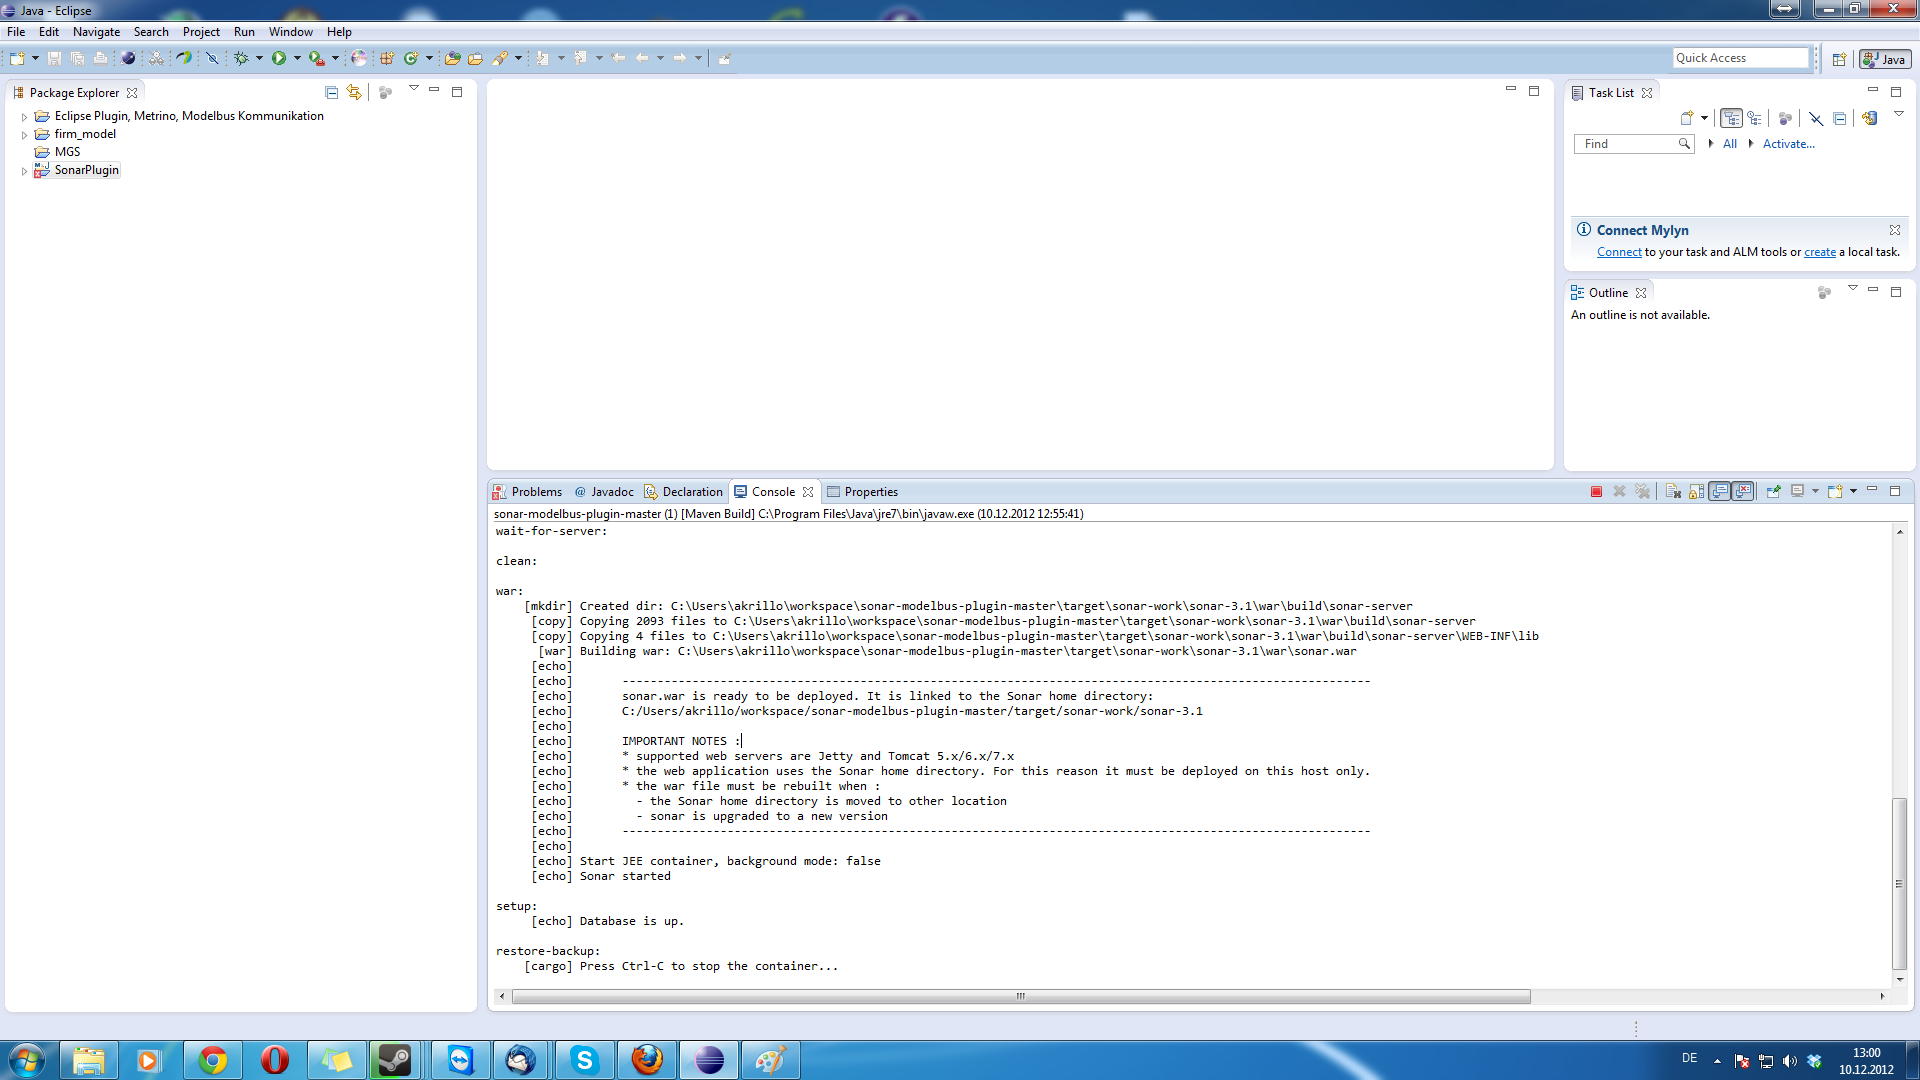
\includegraphics[width=\textwidth]{sonarready}
	\caption{Sonar is ready}
	\label{fig:sonarready}
\end{figure}

Now you can see Sonar running at "localhost:9000"  in your browser.

\begin{figure}
	\centering
		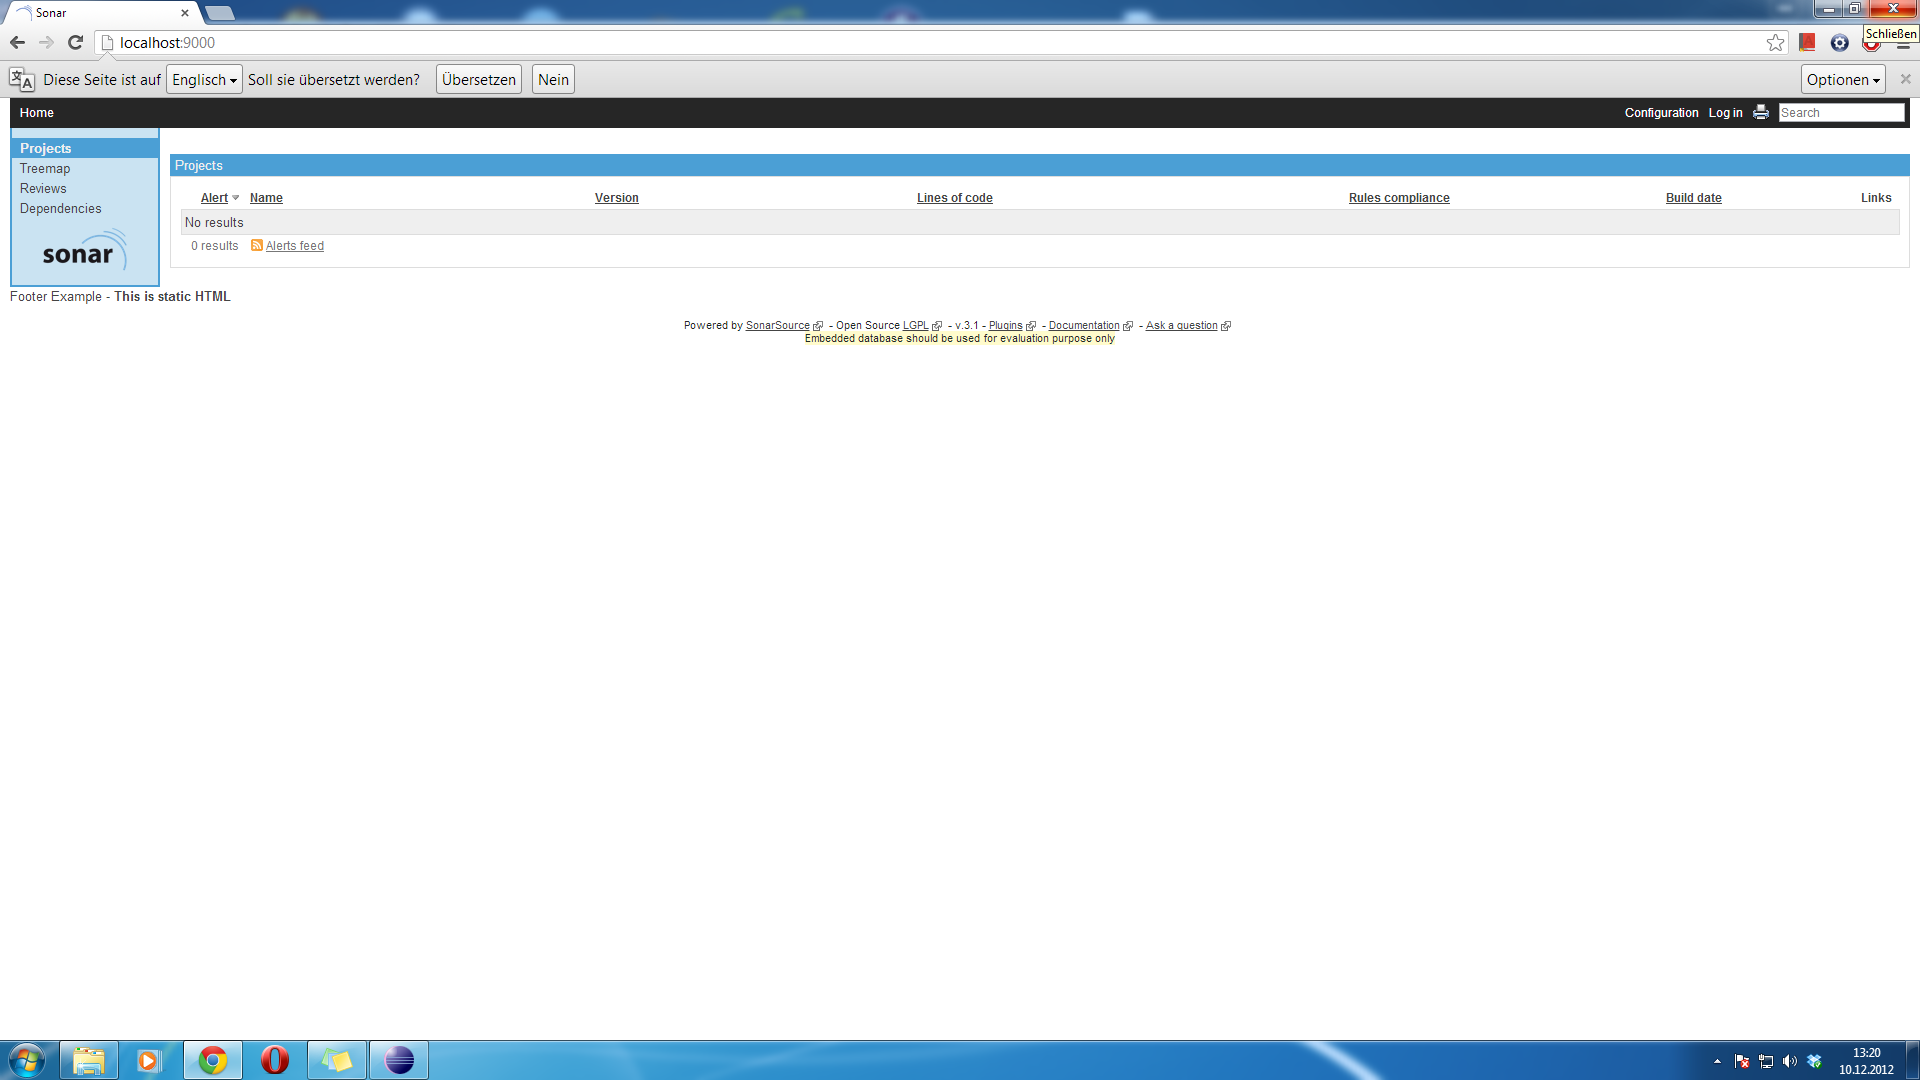
\includegraphics[width=\textwidth]{sonarrunning}
	\caption{Sonar in the browser}
	\label{fig:sonarrunning}
\end{figure}



\subsection{Analysing with Sonar}
If you like to analyse your project with Sonar (or any other Maven project) you can start the build process with the goal "sonar:sonar". After processing you can refresh your browser at "localhost:9000" and can see the results of the analysis.

\begin{figure}
	\centering
		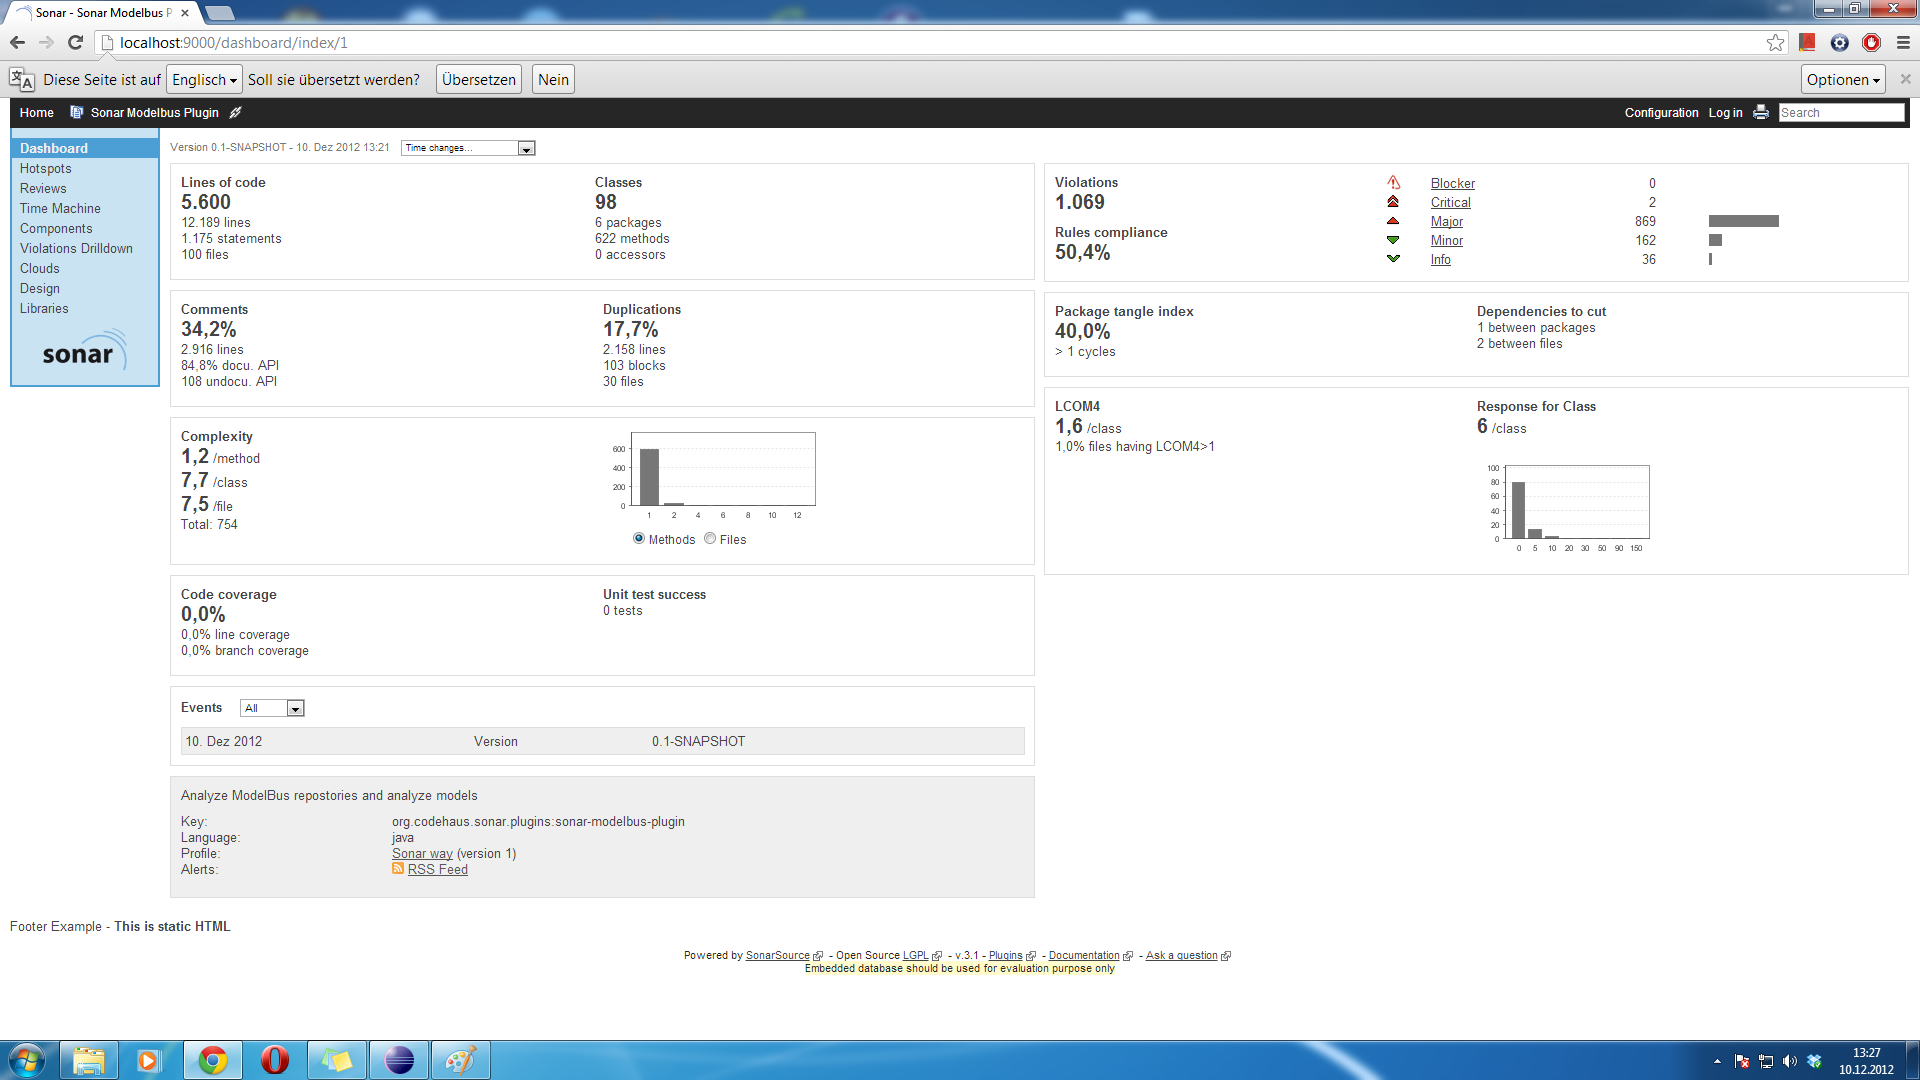
\includegraphics[width=\textwidth]{sonarinaction}
	\caption{Sonar in action}
	\label{fig:sonarinaction}
\end{figure}